Intuitively, the regions within an image that are most salient are likely to have a higher probability of being remembered, since they will draw the attention of viewers and a majority of a viewer’s eye fixations will be spent looking at those regions.. On the other hand, it is conceivable that some visually appealing regions will not be memorable, especially since aesthetic images are known to be less memorable \cite{isola11}, \cite{isola14}. When can visual saliency predict object memorability and what are the possible differences between these two phenomena? Quantifying the precise relationship between saliency and memorability will be paramount  towards understanding object memorability in greater depth.

To this aim, we utilized the eye fixation dataset made available for the Pascal-S dataset in \cite{yin14}. With this dataset in hand, we first calculated the number of unique fixation points within the area of each object and computed the correlation between this metric and the object’s memorability score (Figure \ref{fig:scatterFixation} a). We found this correlation to be positive and considerably high ($\rho = 0.71$), suggesting that fixation count and visual saliency may drive object memorability considerably. However, the large concentration of points on the bottom left part of scatter plot in Figure \ref{fig:scatterFixation} a suggests that part of the reason for this high correlation is that objects that have not been viewed at all have essentially no memorability. Indeed, only objects that have been seen can be remembered. In addition, the points toward the top left appear to decrease in trend. Looking deeper, Figure \ref{fig:fixCorr} plots the change in correlation between object memorability and fixations as the minimum number of fixations inside objects increases. The downward monotonic trend indicates that as the number of fixations inside an object increases, the predictive ability diminishes significantly. In addition, Figure \ref{fig:fixCorr} plots the correlation between object memorability and number of fixations as a function of total number of objects in an image. Similar to the previous trend, as the number of objects in an image increases, the correlation between saliency i.e. number of fixations and memorability score decreases sharply. This finding is in agreement with the two remaining scatter plots in Figure \ref{fig:scatterFixation} b (shows that the memorability of an object decreases in the presence of many other objects) and Figure \ref{fig:scatterFixation} c (shows that number of fixations decreases with the number of objects). This makes intuitive sense since people have more to look at in an image when more objects are present, and so they may look less at any one object, especially if they compete for saliency, and therefore may have a more difficult time remembering those objects.

\begin{figure}[t]
\centering
\subfigure{\centering 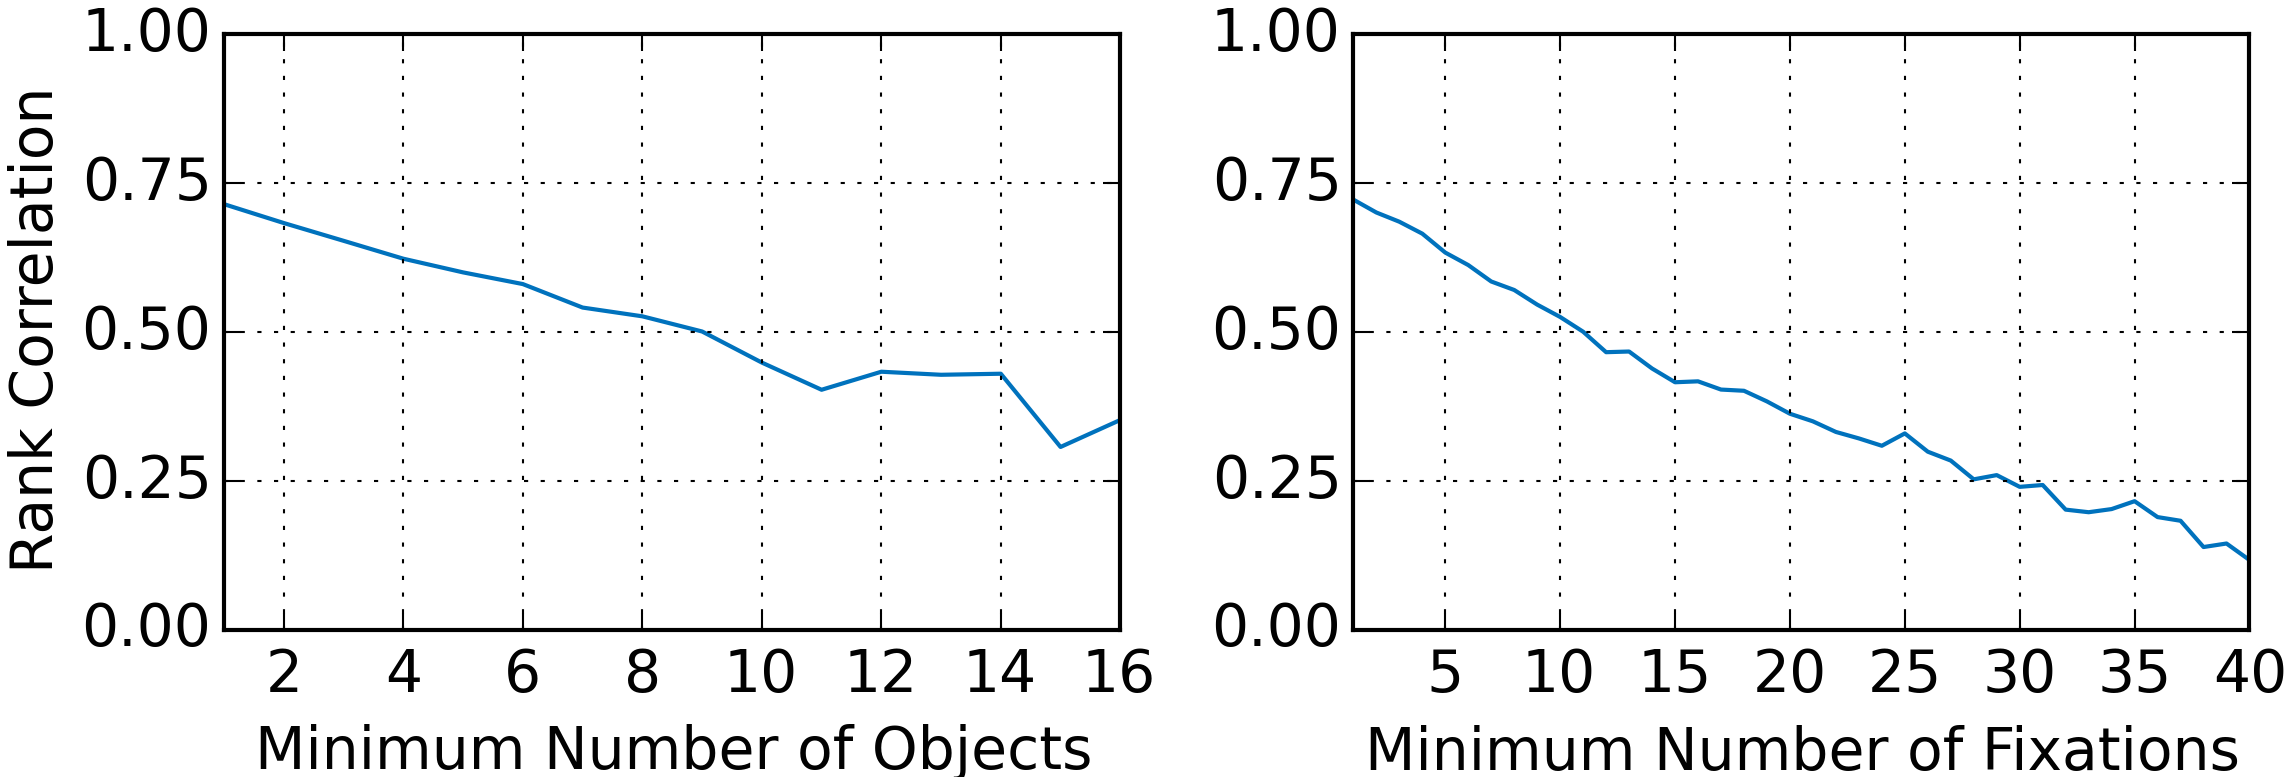
\includegraphics[width=0.5\textwidth]{figures/results/fixation/mem-fix-corr-by-factors.png}}
\vspace{-5mm}\caption{\footnotesize\textbf{Correlation between object memorability and number of fixations.} add-in later. }\label{fig:fixCorr}
\end{figure}

To sum up, saliency is a surprisingly good index of object memorability in simple contexts where there are few objects in the image, or when an object has few interesting points, but it is a much weaker predictor of object memorability in complex scenes containing multiple objects that have many points of interest.

\begin{figure}[b]
\centering
\subfigure{\centering 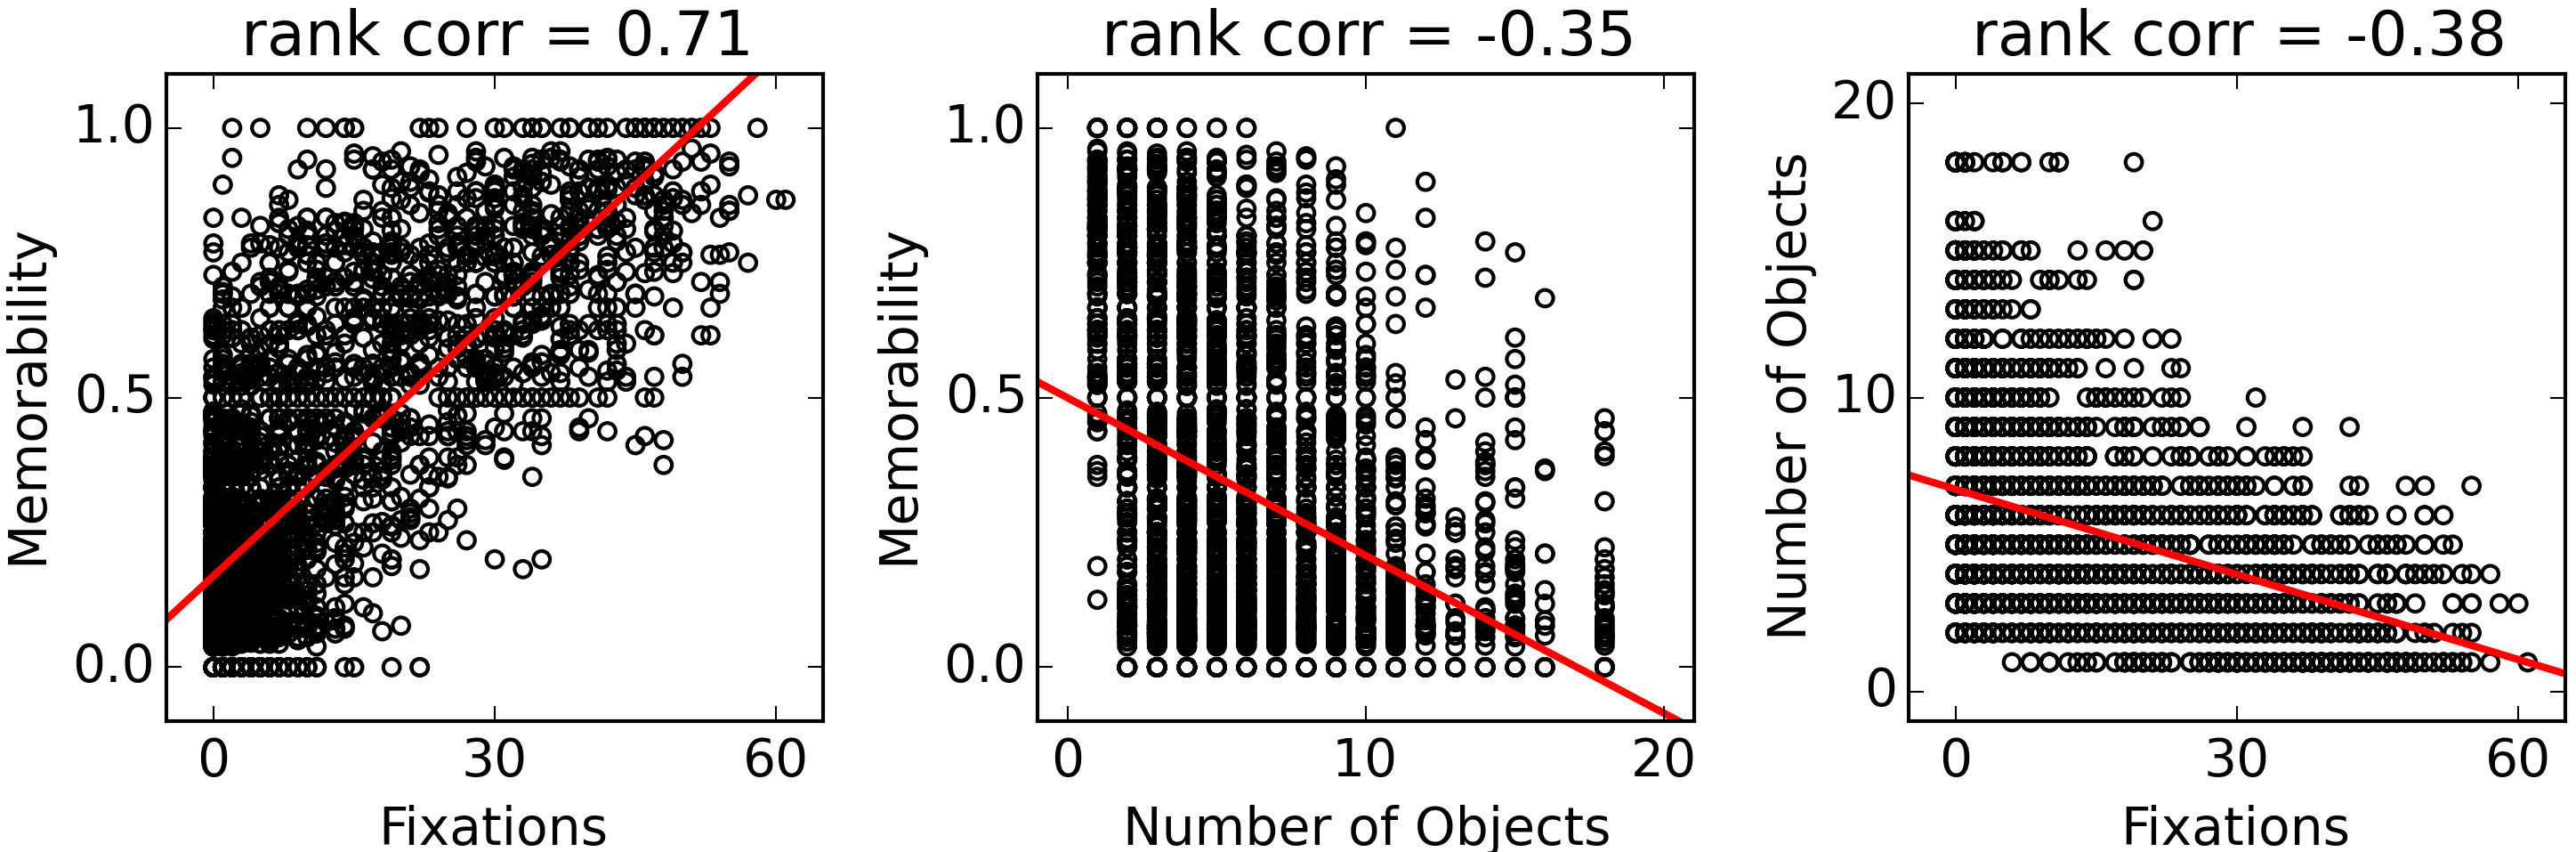
\includegraphics[width=0.5\textwidth]{figures/results/fixation/fix_corr_set.png}}
\vspace{-5mm}\caption{\footnotesize\textbf{Correlation between object memorability and number of fixations.} add-in later. }\label{fig:scatterFixation}
\end{figure}

\textbf{Center Bias: } Figure \ref{fig:fixPos} elucidates another example where saliency and memorability diverge. While previous studies related to visual saliency have showed that saliency is heavily influenced by center bias, Figure \ref{fig:fixPos} shows that memorability exhibits comparatively less center bias than saliency. This is most apparent when considering the difference in the solid ellipse in the right plot (shows where $95\%$ of fixation positions are located), and the dashed ellipse (shows where the $95\%$ of the above-median memorable objects are located).

\begin{figure}[t]
\centering
\subfigure{\centering 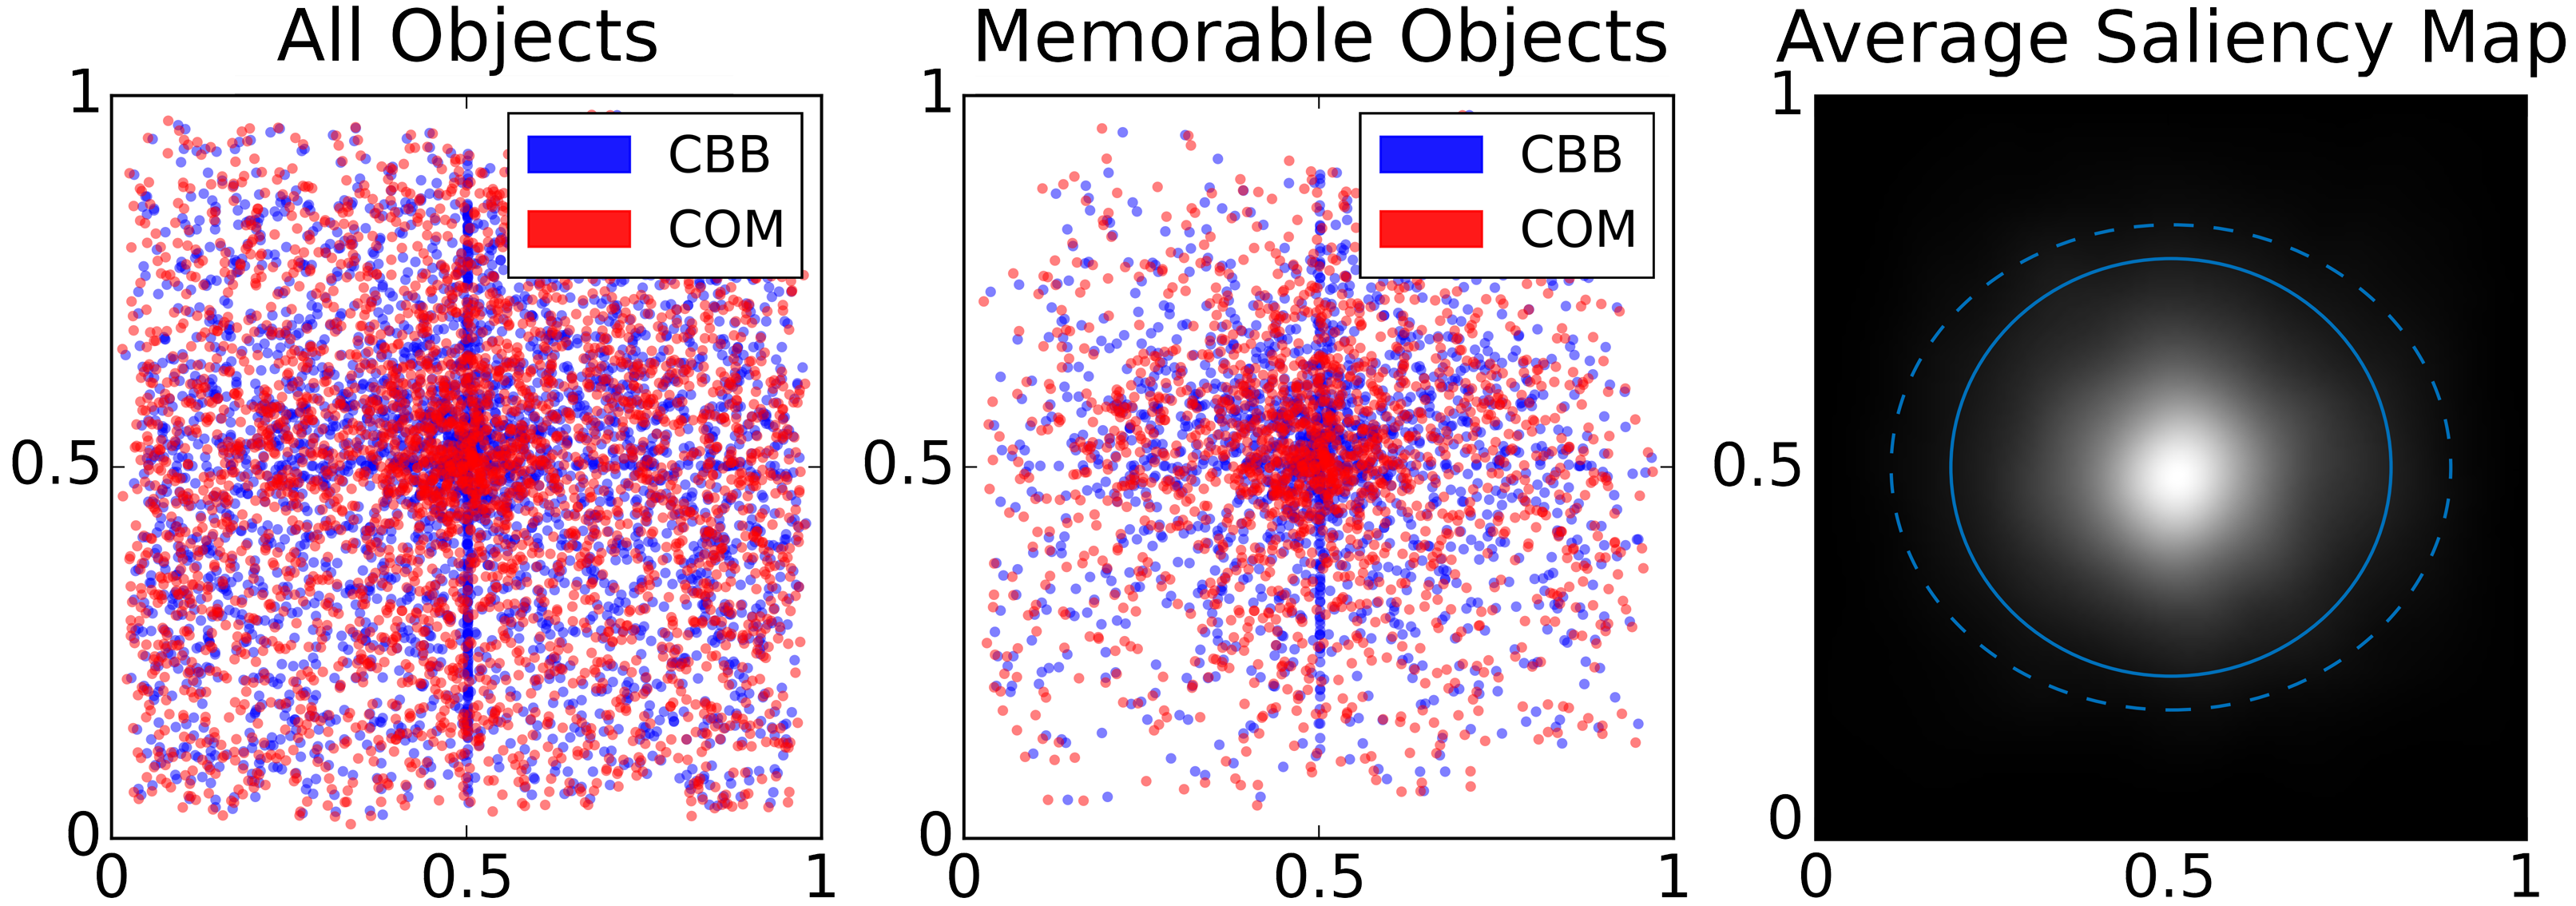
\includegraphics[width=0.5\textwidth]{figures/results/fixation/positions_final.png}}
\vspace{-5mm}\caption{\footnotesize\textbf{Positions.} add-in later. }\label{fig:fixPos}
\end{figure}


